\documentclass{diploma}

\student{Сергеев Владислав Алексеевич}
\group{М8О-411Б-19}
\theme{Разработка клиентской части web-приложения onmp.ru на React}

\supervisor{Пивоваров Дмитрий Евгеньевич}
\firstConsultant{---}
\secondConsultant{---}
\reviewer{---}

\faculty{№ 8 <<Компьютерные науки и прикладная математика>>}
\department{806}
\speciality{02.03.02 <<Фундаментальная информатика и информационные технологии>>}
\profile{Физика}

\departmentFullName{№ 806}
\headOfDepartment{Крылов Сергей Сергеевич}

% Дата. Оставляем пустое место для дня
\date{\uline{\hspace{24pt}} мая \the\year\ года}

\newacronym{api}{API}{Application Programming Interface}
\newacronym{http}{HTTP}{Hypertext Transfer Protocol}
\newacronym{maui}{MAUI}{Multi-platform App UI}
\newacronym{mvvm}{MVVM}{Model-View-ViewModel}
\newacronym{rest}{REST}{Representational State Transfer}
\newglossaryentry{id1}{ % Нужны разные id, можно ставить просто последовательно
    name={Backend},
    description={логика работы сайта, скрытая от пользователя} 
}
\newglossaryentry{id2}{
    name={МКБ},
    description={Международная классификация болезней} 
}
\newglossaryentry{id3}{
    name={$S^{2}$},
    description={формула в списке обозначений} 
}


\addbibresource{main.bib}

% Иллюстрации всегда по центру
\makeatletter
\g@addto@macro\@floatboxreset\centering
\makeatother

\begin{document}
    \maketitle

    % \includepdf[pages=-]{extra/task} % Задание
    \setcounter{page}{2} % Устанавливает счётчик страниц

    \abstract % Структурный элемент: РЕФЕРАТ

 % Реферат

    \tableofcontents % Содержание
    \termsanddefenitions % Термины и определения
    \listofabbreviations % Перечень сокращений и обозначений
 
    \introduction % Структурный элемент: ВВЕДЕНИЕ

Актуальность данной работы связана с необходимостью оптимизации процесса работы врачей из отделения неотложной медицинской помощи, особенно тех, которые выезжают на вызовы с использованием машин скорой помощи. В настоящее время эти медицинские специалисты заполняют бумажные карты вызова во время осмотра пациента на дому. Однако, такой подход требует ношения с собой больших объемов бумажной документации, что требует больших затрат времени и ресурсов на их заполнение, обработку и хранение.

Переход к электронному заполнению карт вызова имеет ряд значительных преимуществ. Прежде всего, медицинским работникам будет значительно удобнее носить с собой меньшее количество объемной макулатуры, так как электронная форма позволит им быстро и удобно заполнять карты вызова с использованием мобильных устройств, которые они всегда имеют под рукой. Это значительно повысит мобильность и гибкость работы медицинского персонала, позволяя им быстро и эффективно заполнять и обрабатывать данные.

Второе преимущество заключается в возможности хранения электронных карт вызова в интернете. Вместо физического хранения и поиска бумажных документов, медицинские работники смогут сохранять все карты вызова в электронном виде, обеспечивая быстрый и удобный доступ к ним из любого места. Это также позволит легко распечатывать необходимые карты вызова в случае необходимости, например, для передачи другим специалистам или для ведения медицинской документации.

Основной целью данной работы является разработка клиентской части web-сервиса с использованием технологии React.js. Это позволит создать современный и интуитивно понятный пользовательский интерфейс, который облегчит заполнение карт вызова, ускорит процесс ввода данных и повысит эффективность работы медицинских работников.

Был проведен анализ требований к функциональности и пользовательскому интерфейсу web-сервиса, разработана архитектура решения, реализованы необходимые компоненты и проведено тестирование системы. Также была осуществлена интеграция клиентской части с серверной частью системы для обеспечения полной функциональности и взаимодействия с данными.

В рамках данной исследовательской работы можно определить следующие задачи:
\begin{itemize}
    \item Анализ требований к клиентской части web-сервиса: Эта задача включает в себя изучение требований, предъявляемых заказчиком к функциональности и дизайну клиентской части web-сервиса. Необходимо провести тщательный анализ требований, чтобы полноценно понять ожидания и потребности заказчика.
    \item Проектирование клиентской части: Включает разработку детального плана и архитектуры клиентской части web-сервиса. Эта задача включает определение структуры компонентов, взаимодействия между ними, выбор подходящих библиотек и фреймворков для разработки, а также определение способа организации данных и обработки событий.
    \item Разработка функционала авторизации и аутентификации: Данный функционал позволит медицинским работникам входить в систему с использованием уникальных учетных данных. Каждому пользователю будет предоставлен доступ к рабочей среде, где они смогут создавать и использовать собственные шаблоны, а также просматривать и заполнять свои собственные карты вызова.
    \item Создание интерфейса для заполнения и сохранения карт вызова: Разработка пользовательского интерфейса, позволяющего медицинским работникам вводить информацию о состоянии здоровья пациента, тем самым заполняя карту вызова. Данные должны быть легко вводимы и интуитивно понятны, чтобы ускорить процесс заполнения.
    \item Реализация функционала хранения и организации карт вызова в папках: Готовые, Незавершенные, Архив, Шаблоны. Для организации и удобного отображения карт вызова. Это позволит медицинским работникам быстро найти и просмотреть необходимые карты вызова в соответствующих категориях.
    \item Разработка функционала создания и использования шаблонов: Реализация возможности создания шаблонов для быстрого использования частично заполненных карт вызова. Создавая шаблон, пользователь заполняет только некоторые поля карты, чтобы в дальнейшем использовать данный шаблон как основу для карты вызова.
    \item Реализация Функционала поиска, группировки и сортировки карт вызова: Предоставление возможности быстрого поиска нужной информации на основе различных параметров, таких как дата, название карты. Кроме того, группировка и сортировка карт вызова позволят легко ориентироваться в большом объеме данных, что значительно упростит процесс поиска нужной информации.
    \item Тестирование и отладка системы: Проведение тестирования для проверки функциональности и корректности работы системы. Исправление ошибок и устранение неполадок для обеспечения стабильной работы web-сервиса.
\end{itemize}


В данной работе разработка клиентской части web-сервиса осуществляется с использованием React.js - популярной JavaScript-библиотеки для построения пользовательских интерфейсов. React.js предоставляет эффективные инструменты и подходы для создания интерактивных веб-приложений с удобной обработкой данных и переиспользуемыми компонентами. Данная библиотека базируется на концепции компонентного подхода, где пользовательский интерфейс разбивается на независимые компоненты, каждый из которых может иметь свою логику и состояние. Компоненты могут быть переиспользованы, что упрощает разработку и обслуживание приложения.

Дополнительным инструментом к React был выбран Redux. Это библиотека JavaScript, которая предоставляет инструменты для управления состоянием приложения. Она является популярным выбором для разработки сложных и масштабируемых приложений, особенно тех, которые имеют большое количество взаимосвязанных данных.

Redux основывается на концепции однонаправленного потока данных и централизованного хранилища состояния. Вместо того чтобы хранить состояние внутри компонентов, Redux предлагает вынести состояние в отдельное хранилище. Компоненты могут получать доступ к состоянию из хранилища и обновлять его, используя специальные функции.

В целом, совместное использование React и Redux позволяет создавать масштабируемые, предсказуемые и легко поддерживаемые приложения с удобным управлением состоянием \cite{React&Redux}. 

Помимо этого, был выбрана библиотека Axios, которая предоставляет удобный интерфейс для выполнения HTTP-запросов из браузера. Она позволяет взаимодействовать с внешними API, отправлять запросы на сервер и обрабатывать полученные ответы.

Главная цель Axios - упростить и сделать более эффективной работу с HTTP-запросами. Она предоставляет простые методы для отправки различных типов запросов, таких как GET, POST, PUT, DELETE и другие. Кроме того, Axios предоставляет возможности для установки заголовков запроса, обработки ошибок, использования интерсепторов и других функций.

Разработка данного сервиса основывалась на архитектурной методологии Feature-Sliced Design, которая помогает структурировать код и организовать проект на основе функциональных возможностей. Она призвана улучшить масштабируемость, переиспользуемость и поддерживаемость кодовой базы. Основная идея данной методологии заключается в том, что проект разбивается на слои, каждый из которых имеет свою "зону ответственности". Каждый модуль содержит все необходимые компоненты, состояние, стили и логику, связанные с этой функциональностью. Это позволяет разработчикам работать над каждой фичей независимо друг от друга.

Результатом данной работы будет функциональный web-сервис, предоставляющий возможность электронного заполнения и хранения карт вызова для медицинских работников из отделения неотложной помощи. Ожидается, что данное решение значительно улучшит процесс работы медицинских учреждений, сократит временные затраты на бумажную работу и повысит качество медицинской помощи пациентам.

Таким образом, данная дипломная работа имеет практическую значимость и является важным шагом в совершенствовании сферы оказания неотложной медицинской помощи, предлагая инновационное решение, которое отсутствует на рынке.
 % Введение

    \section{ПОТРЕБНОСТЬ В РАЗРАБОТКЕ}

\subsection{Анализ текущих методов заполнения и хранения карт вызова}

В настоящее время, при вызове скорой помощи, медики используют методические пособия и бланки карт вызова, которые хранятся в объемной папке.

Метод заполнения карт вызова имеет свои особенности. В зависимости от состояния пациента, медики заполняют различные разделы карты, начиная от основной информации о пациенте и заканчивая деталями о его состоянии, симптомах и проведенных медицинских процедурах.

Для правильного заполнения карт вызова медицинскими работниками требуется знание определенных протоколов и стандартов. Для этого они обычно имеют с собой несколько методических пособий, содержащих инструкции по заполнению различных разделов карты вызова в зависимости от состояния пациента. Это усложняет процесс и требует дополнительного времени и усилий. Помимо этого, медицинские работники заполняют карты вызова в процессе осмотра пациента. Это требует их присутствия и внимания к пациенту, а также необходимости записывать информацию вручную.

Хранение карт вызова также имеет свои особенности. Обычно эти документы хранятся в специальных папках или ящиках машины скорой помощи, доступных только медицинским работникам, которые после окончания смены передаются отделению в медицинском учреждении для формирования отчетности. Это создает дополнительный вес и занимает место в машине скорой помощи, а также создаёт проблемы с доступом к предыдущим записям и усложняет поиск и извлечение информации о конкретных пациентах или случаях. 

Однако, существуют и недостатки текущих методов заполнения и хранения карт вызова. Например, при использовании бумажных бланков возможны ошибки в заполнении или потеря документов. Кроме того, доступ к картам вызова может быть ограничен, что затрудняет своевременное и эффективное оказание медицинской помощи.

В связи с этим, возникает потребность в новых технологиях, которые позволят ускорить процесс заполнения карт вызова, уменьшить количество ошибок и обеспечить безопасное хранение этих документов. Таким образом разработка web-сервиса, позволяющего заполнять карты вызова в электронной форме, представляет собой актуальное и необходимое решение для улучшения и оптимизации процесса работы медицинских работников из отделения неотложной медицинской помощи.

В целом, анализ текущих методов заполнения и хранения карт вызова показал, что они имеют свои преимущества и недостатки. Но в современном мире, где ценится скорость и качество медицинской помощи, возникает потребность в новых технологиях, которые помогут повысить эффективность работы медицинских работников и обеспечить быстрое и точное оказание помощи пациентам.

\subsection{Описание проблем и ограничений существующих решений}

Анализируя существующие решения, такие как сайт-прототип заполнения карт вызова onmp.ru, представленный на рисунке~\ref{fig:onmp-prototype},

\begin{figure}
  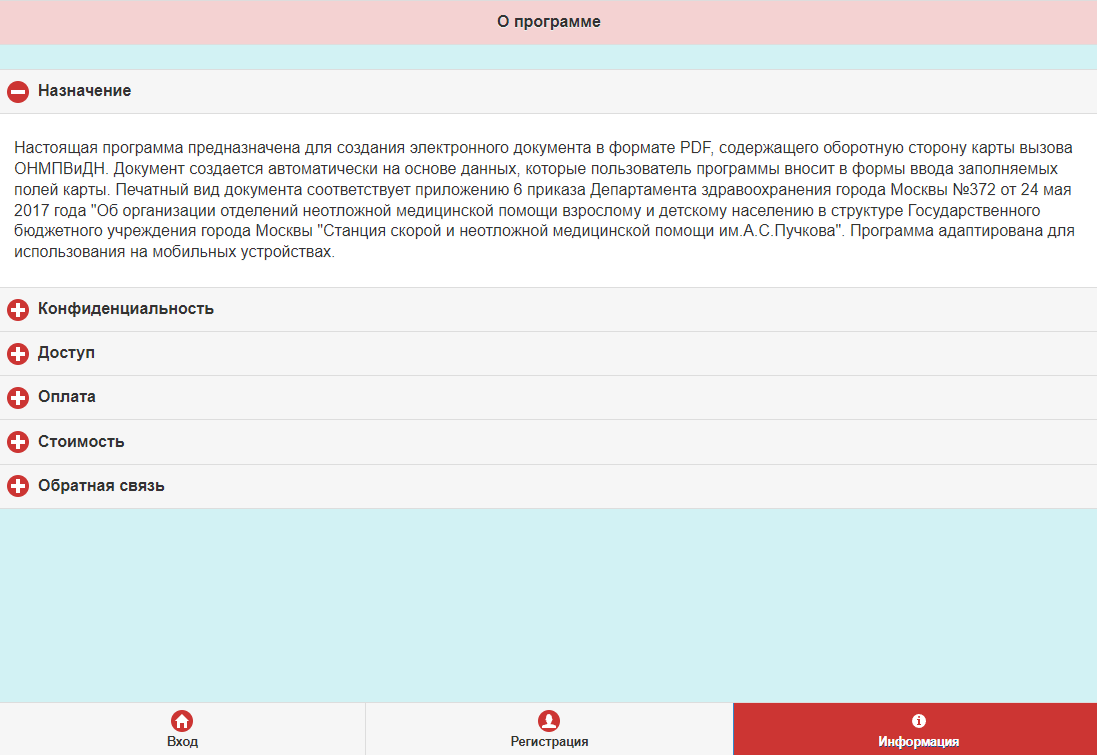
\includegraphics[scale=0.5]{styles/diploma/inc/onmp-prototype.png}
  \caption{Сайт-прототип onmp.ru}
  \label{fig:onmp-prototype}
\end{figure}
можно выделить несколько проблем и ограничений, которые ограничивают его удобство использования и эффективность:

Язык программирования PHP: Использование PHP для разработки сайта может ограничивать его гибкость и масштабируемость. PHP является языком серверной разработки, и его использование может усложнить внесение изменений и расширение функциональности клиентской части.

Неудобный UX-дизайн: Отсутствие интуитивного и удобного UX-дизайна на сайте может создавать сложности при навигации между разделами, а также затруднять быстрый доступ к нужной информации. Неочевидные переходы и отсутствие удобной навигации могут снижать эффективность работы мед.работников и увеличивать время заполнения карт вызова.

Отсутствие промежуточного сохранения: Наличие функции промежуточного сохранения карт вызова является важным аспектом для удобства пользователей. Отсутствие такой функции на сайте может приводить к потере данных в случае прерывания работы или случайного закрытия страницы.

Ограниченные возможности навигации по карте: Отсутствие быстрой навигации по карте вызова может затруднять поиск и редактирование определенных разделов или полей, особенно в случае больших и сложных карт.

Учитывая эти проблемы и ограничения существующего решения, разработка нового web-сервиса для заполнения карт вызова с использованием React.js имеет потенциал для устранения данных проблем и предоставления более удобного и эффективного инструмента для медицинских работников из отделения неотложной помощи.

\subsection{Обзор преимуществ перехода на электронную форму заполнения карт вызова}

Переход на электронную форму заполнения и хранения карт вызова имеет несколько преимуществ. 

\begin{itemize}
    \item Использование электронной формы позволяет существенно сократить потребление бумаги и уменьшить негативное влияние на окружающую среду. Это способствует экологической устойчивости и снижению расходов на закупку и хранение бумажных материалов.
    \item Электронная форма позволяет быстро и удобно заполнять карты вызова, что ведет к повышению эффективности работы медицинских работников. Заполнение осуществляется путем выбора и ввода данных в соответствующие поля, что сокращает время, затрачиваемое на ручное заполнение бумажных форм.
    \item Электронная форма обеспечивает легкий доступ к заполненным картам вызова из любого места с подключением к Интернету. Это позволяет медицинскому персоналу быстро получать необходимую информацию о пациентах, это особенно полезно для медицинских работников, которые находятся в пути, например, в машине скорой помощи. Они могут легко получить доступ к системе и заполнить карты вызова на своих устройствах. Также электронна форма облегчает анализ и обработку данных для статистической отчетности и исследований. Помимо этого, медицинский персонал может получить доступ к предыдущим записям о состоянии пациента и процедурах, которые ему проводились, что помогает улучшить качество медицинской помощи и сделать более точный диагноз.
    \item При использовании электронной формы можно внедрить функциональность автоматического заполнения и проверки данных. Например, система может предложить автозаполнение некоторых полей на основе предыдущих записей или данных из других систем, а также проводить проверку на наличие ошибок или недостаточных данных.
    \item Электронные карты вызова могут быть сохранены в централизованной базе данных, что облегчает их архивирование и поиск. Можно использовать различные фильтры и категории для организации и классификации карт по статусу (готовые, незавершенные, архив) или другим параметрам, упрощая их управление и обработку.
    \item В электронной форме можно создавать шаблоны часто используемых или стандартных карт вызова. Это позволяет медицинскому персоналу быстро заполнять карты, используя предварительно сохраненные данные, что повышает производительность и снижает вероятность ошибок.
\end{itemize}

Переход на электронную форму заполнения карт вызова значительно сокращает бумажную работу, повышает эффективность и точность процесса заполнения, улучшает доступность и хранение данных, а также облегчает анализ и управление информацией. Это современный и инновационный подход, который может значительно улучшить работу мед.работников и повысить качество оказываемой медицинской помощи.

    \section{АНАЛИЗ ТРЕБОВАНИЙ ЗАКАЗЧИКА К ФУНКЦИОНАЛЬНОСТИ И ДИЗАЙНУ}

\subsection{Описание требований к интерфейсу заполнения карт вызова}

Эффективное и надежное заполнение карт вызова является важным процессом для медицинских работников, поскольку это напрямую влияет на качество медицинской помощи. Интерфейс, который будет использоваться для заполнения карт вызова, должен быть специально разработан, чтобы обеспечить максимальную эффективность и удобство использования.

Для удовлетворения этих требований заказчиком было предложено несколько критериев, которым должен соответствовать медицинский интерфейс:

\begin{itemize}
    \item Интерфейс должен быть легким в освоении и использовании даже для пользователей с минимальными навыками работы с компьютером. Он должен предоставлять понятные и логично расположенные элементы управления, а также ясные инструкции для заполнения каждого поля.
    \item Интерфейс должен быть организован логически, с ясной и понятной структурой разделов и подразделов, отражающих последовательность заполнения карты вызова. Навигация должна быть интуитивной и обеспечивать быстрый переход между разделами, чтобы медицинскому работнику было удобно перемещаться по карте вызова.
    \item Интерфейс должен предоставлять функциональность сохранения заполненной информации, чтобы медицинским работникам не приходилось вводить одни и те же данные снова и снова при каждом новом вызове. Также желательно наличие функции автозаполнения полей на основе предыдущих записей или шаблонов.
    \item Интерфейс должен быть адаптивным и оптимизированным для работы на различных устройствах, включая компьютеры, планшеты и смартфоны. Это обеспечит удобство использования сервиса как в офисной среде, так и на мобильных платформах, когда медицинские работники находятся на вызове.
    \item Интерфейс должен предоставлять возможность интеграции с дополнительными функциональностями, которые помогут медицинским работникам в процессе заполнения карты вызова. Например, он может предоставлять доступ к алгоритмам оказания помощи, таблицам дифференциальной диагностики, калькуляторам дозировок и справочникам, которые помогут в принятии решений и заполнении необходимых полей.
\end{itemize}

\subsection{Рассмотрение требований к организации папок и шаблонов карт вызова}

При организации папок и шаблонов карт вызова, необходимо учитывать множество требований для обеспечения максимальной эффективности и удобства использования.

В первую очередь, необходимо установить четыре папки хранения карт вызова: Готовые, Незавершенные, Архив и Шаблоны.

В папку Готовые попадают карты после того, как пользователь заполнит все необходимые поля на карте вызова и нажмет кнопку "Сохранить". Это позволяет пользователю быстро найти уже готовые карты вызова и не тратить время на поиск незавершенных карт.

В папку Незавершенные попадают карты, когда пользователь возвращается в каталог карт, закрывает вкладку или не нажимает кнопку "Сохранить". При этом, уже заполненные данные сохраняются в процессе заполнения в базу данных, чтобы пользователь мог продолжить заполнение карты вызова с того места, где он остановился. Это позволяет избежать потери уже заполненных данных и повторного заполнения всех полей заново.

В папку Архив попадают карты после того, как они были распечатаны. Это гарантирует сохранность уже готовых карт вызова, которые могут понадобиться в будущем для анализа статистики и других целей.

Папка Шаблоны предоставляет дополнительный функционал создания шаблона с частичным заполнением полей карты вызова. Это позволяет пользователям создавать базовые шаблоны карт вызова, которые можно использовать в будущем как основу для новых карт вызова. Это значительно ускоряет процесс заполнения карт вызова, так как многие поля уже будут заполнены заранее.

Такая организация папок и шаблонов карт вызова обеспечит удобство хранения, поиска и использования карт, а также улучшит процесс работы медицинского персонала, обеспечивая быстрый доступ к необходимым данным и возможность повторного использования шаблонов.

Дополнительные требования к функциональности организации папок и шаблонов карт вызова:

Сортировка по дате:

\begin{itemize}
    \item Возможность сортировки карт вызова внутри каждой папки по дате их создания или последнего изменения.
    \item Медицинским работникам предоставляется возможность выбора порядка сортировки (по возрастанию или убыванию даты).
\end{itemize}

Сортировка по названию карты:

\begin{itemize}
    \item Возможность сортировки карт вызова внутри каждой папки по их названию.
    \item Медицинским работникам предоставляется возможность выбора порядка сортировки (по алфавиту, по возрастанию или убыванию).
\end{itemize}

Группировка:

\begin{itemize}
    \item Возможность группировки карт вызова по определенным параметрам, например, по дате и названию карты.
    \item Медицинским работникам предоставляется возможность выбора группировки и просмотра карт вызова внутри каждой группы.
\end{itemize}

Реализация сортировки и группировки в каждой папке улучшит удобство работы с картами вызова, позволит пользователю быстро находить нужную информацию и эффективно управлять списками карт. Это значительно повысит эффективность работы и улучшит пользовательский опыт.

    \section{ТЕХНОЛОГИЧЕСКИЙ СТЕК И АРХИТЕКТУРНАЯ МЕТОДОЛОГИЯ}

\subsection{Обоснование выбора React.js в качестве основной технологии разработки}
\subsubsection{Обзор существующих технологий и фреймворков}

При разработке клиентской части web-сервисов существует несколько популярных технологий и фреймворков, которые предоставляют разработчикам средства для создания интерактивных и отзывчивых пользовательских интерфейсов. В данном разделе мы рассмотрим три из них: Angular, Vue.js и React.js.

Angular - это фреймворк, разработанный компанией Google. Он использует язык программирования TypeScript и предоставляет набор инструментов для создания масштабируемых приложений \cite{Angular}. 

Основные особенности Angular:

\begin{itemize}
    \item компонентная архитектура: Angular основан на компонентах, которые являются основными строительными блоками приложения. Компоненты позволяют создавать переиспользуемые элементы интерфейса и упрощают управление состоянием;
    \item двустороннее связывание данных: Angular предлагает двустороннее связывание данных, что позволяет автоматически синхронизировать данные между моделью и представлением;
    \item мощный набор инструментов: Angular предоставляет широкий спектр инструментов для разработки, таких как маршрутизация, формы, валидация, анимации и многое другое;
    \item строгая типизация: TypeScript, язык программирования, используемый Angular, предлагает статическую типизацию, что улучшает безопасность и облегчает разработку сложных приложений;
\end{itemize}

Vue.js - это прогрессивный JavaScript-фреймворк с открытым исходным кодом. Он создан для разработки пользовательских интерфейсов и может быть поэтапно внедрен в существующие проекты \cite{Vue.js}. 

Основные особенности Vue.js:

\begin{itemize}
    \item простота и гибкость: Vue.js предлагает простой и интуитивно понятный API для создания компонентов и управления состоянием. Он также обладает гибкостью, позволяющей использовать только необходимые части фреймворка;
    \item реактивность: Vue.js использует систему реактивности, которая автоматически обновляет пользовательский интерфейс при изменении данных;
    \item однофайловые компоненты: Vue.js позволяет создавать компоненты с помощью одного файла, включающего шаблон, скрипт и стили. Это делает разработку и поддержку компонентов более организованной и удобной;
    \item экосистема и сообщество: Vue.js имеет активное сообщество разработчиков и обширную экосистему плагинов и инструментов, которые упрощают разработку и расширение функциональности;
\end{itemize}

React - это JavaScript-библиотека, разработанная Meta (Компания признана экстремистской и запрещенной в России). Она используется для создания пользовательских интерфейсов и часто применяется в разработке одностраничных приложений \cite{React.js}. 

Основные особенности React:

\begin{itemize}
    \item компонентный подход: React основан на компонентах, которые позволяют создавать переиспользуемые элементы интерфейса. Компоненты в React обладают своим состоянием и жизненным циклом, что упрощает разработку и поддержку приложений;
    \item виртуальный DOM: React использует виртуальный DOM, который позволяет эффективно обновлять только измененные части пользовательского интерфейса, что повышает производительность;
    \item односторонний поток данных: В React данные передаются через props от родительских компонентов к дочерним. Это делает управление состоянием более предсказуемым и упрощает отладку;
    \item большое сообщество и экосистема: React имеет широкое сообщество разработчиков и богатую экосистему инструментов, библиотек и компонентов, которые облегчают разработку и ускоряют процесс создания приложений;
\end{itemize}

\subsubsection{Преимущества React.js}

При выборе основной технологии разработки для клиентской части web-сервиса было принято решение использовать React.js. Рассмотрим основные аргументы и преимущества, которые оказали влияние на это решение:

\begin{itemize}
    \item React.js является одной из самых популярных JavaScript-библиотек для создания пользовательских интерфейсов. Он активно используется множеством компаний и разработчиков по всему миру. Большое сообщество разработчиков React способствует обмену знаниями, наличию документации, обновлениям и поддержке.
    \item React.js предлагает гибкую и модульную архитектуру разработки. Он позволяет создавать компоненты, которые могут быть переиспользованы и управляться независимо друг от друга. Это упрощает разработку сложных пользовательских интерфейсов и облегчает сопровождение кода.
    \item React.js использует виртуальный DOM, который является эффективным механизмом обновления только измененных частей пользовательского интерфейса. Это приводит к улучшенной производительности и отзывчивости приложения, особенно при работе с большими объемами данных.
    \item React.js обладает богатой экосистемой инструментов, библиотек и компонентов, которые могут быть использованы для ускорения разработки. Наличие таких инструментов, как Redux для управления состоянием, React Router для маршрутизации, Styled Components для стилизации и многих других, делает разработку более эффективной и продуктивной.
    \item React.js обеспечивает хорошую тестируемость кода благодаря своей компонентной архитектуре. Тестирование компонентов React может быть проведено с использованием различных инструментов и библиотек, таких как Jest или Enzyme. Это позволяет обеспечить высокую степень надежности и качества разрабатываемого приложения.
    \item React.js поддерживается активным сообществом разработчиков и командой Facebook. Это гарантирует наличие обновлений, исправлений ошибок и новых возможностей. Кроме того, Facebook активно продвигает и разрабатывает новые инструменты и библиотеки в рамках экосистемы React.
\end{itemize}

Исходя из этих преимуществ и аргументов, выбор React.js в качестве основной технологии разработки для клиентской части web-сервиса является обоснованным и позволит нам создать современное, масштабируемое и эффективное приложение.

\subsection{Описание используемых инструментов}

\subsubsection{React Router}

React Router является мощным инструментом для управления маршрутизацией веб-приложений на платформе React. Он предоставляет удобные и гибкие средства для определения и управления различными маршрутами приложения, позволяя пользователям перемещаться между различными страницами и взаимодействовать с контентом.

Основной концепцией в React Router является использование компонента <Route>. Каждый <Route> определяет отдельный маршрут и указывает, какой компонент должен быть отображен при соответствии данному маршруту. Например, <Route path="/calculator" component={Calculator} /> означает, что при обращении к маршруту "/calculator" будет отображаться компонент Calculator.

Для создания ссылок между страницами используется компонент <Link>. Он позволяет создавать кликабельные элементы, которые перенаправляют пользователя на другие маршруты приложения. <Link to="/calculator">Calculator</Link> создает ссылку на маршрут "/calculator", при нажатии на которую пользователь будет перенаправлен на страницу Calculator.

Для работы с динамическими параметрами в URL, такими как идентификаторы или другие переменные, React Router предлагает использовать параметризованные маршруты. Например, <Route path="/users/:id" component={User} /> определяет маршрут, включающий динамический параметр ":id". Значение этого параметра может быть извлечено в компоненте User с помощью хука useParams().

React Router также предоставляет механизм вложенных маршрутов. Это позволяет создавать иерархическую структуру маршрутов, где определенные компоненты могут быть вложены в другие компоненты и иметь свои собственные подмаршруты. Это особенно полезно для создания сложных макетов приложений с различными уровнями вложенности.

Помимо основных компонентов, React Router также предлагает другие полезные возможности, такие как редиректы, защита маршрутов с помощью приватных роутов, анимации переходов между страницами и многое другое.

Одним из главных преимуществ React Router является его простота использования и интеграция с экосистемой React. Он предоставляет удобные и понятные API, что делает его доступным для разработчиков всех уровней опыта. Благодаря модульной архитектуре React Router, компоненты и маршруты могут быть легко переиспользованы и поддерживаемыми, что способствует быстрой разработке и поддержке приложения.

В заключение, React Router - это мощный инструмент, который значительно облегчает управление маршрутизацией веб-приложений на платформе React. Он предоставляет удобные и гибкие средства для определения маршрутов, создания ссылок и обработки динамических параметров. Благодаря своей простоте использования и интеграции с экосистемой React, React Router является популярным выбором для разработки масштабируемых и гибких веб-приложений.

\subsubsection{Redux}

Redux - это популярная библиотека управления состоянием для JavaScript-приложений, в том числе для приложений, созданных с использованием фреймворка React. Она предоставляет эффективные средства для организации и управления состоянием приложения, делая его предсказуемым и легко поддерживаемым.

Основной концепцией Redux является единственный источник истины - единое хранилище данных, которое содержит всю информацию, необходимую для работы приложения. Вся информация хранится в виде неизменяемого объекта, который называется "состояние". Состояние приложения не может быть изменено напрямую, а только через специальные функции, называемые "редьюсеры".

Редьюсеры - это чистые функции, которые принимают текущее состояние и действие, и возвращают новое состояние на основе этих данных. Они определяют, как должно измениться состояние приложения в ответ на определенные действия. Redux обеспечивает простой и предсказуемый поток данных, где состояние всегда обновляется с помощью редьюсеров.

Один из ключевых элементов Redux - это диспетчер, который является интерфейсом для отправки действий в хранилище. Действия - это простые объекты, которые описывают, что произошло в приложении. Диспетчер принимает действия и передает их в редьюсеры, которые в свою очередь обновляют состояние приложения.

Для удобного использования Redux в приложении, React-компоненты могут подписываться на изменения состояния и получать необходимые им данные из хранилища. Это достигается с помощью специального компонента высшего порядка (Higher-Order Component) или с помощью хука useSelector в React Redux.

Кроме основных концепций, Redux предлагает ряд дополнительных возможностей для упрощения разработки. Например, с помощью middleware можно добавить дополнительные функциональности к обработке действий, такие как асинхронные запросы или логирование. Redux также обеспечивает инструменты для отладки, позволяющие просматривать историю действий и состояния приложения во время разработки.

Одним из главных преимуществ Redux является его способность обрабатывать сложные состояния приложения и поддерживать их расширение в будущем. Он способствует предсказуемости и тестируемости кода, а также упрощает сопровождение и отладку приложения.

В заключение, Redux является мощным инструментом для управления состоянием в JavaScript-приложениях, особенно в сочетании с React. Он предоставляет эффективные средства для организации и обновления состояния, делая приложение более предсказуемым и легко поддерживаемым. Redux позволяет создавать масштабируемые и гибкие приложения, которые легко расширять и изменять в будущем.

\subsubsection{Axios}

Axios - это популярная библиотека для выполнения HTTP-запросов из JavaScript-приложений. Она предоставляет удобный и гибкий интерфейс для взаимодействия с сервером, обеспечивая простоту в использовании и мощные функциональные возможности.

Одной из главных причин популярности Axios является его простота в настройке и использовании. Для отправки HTTP-запроса с помощью Axios необходимо всего несколько строк кода. Библиотека предоставляет функции для различных типов запросов, таких как GET, POST, PUT, DELETE, и др., а также для отправки данных в формате JSON, форм-данных или в виде файлов. Это делает процесс взаимодействия с сервером интуитивно понятным и удобным для разработчиков.

Одной из ключевых особенностей Axios является поддержка Promise API. Он возвращает Promise-объект, что позволяет использовать синтаксис async/await для управления асинхронными операциями. Это упрощает обработку ответов от сервера и выполнение последовательных запросов.

Axios также обладает мощными возможностями по обработке ошибок и перехвату запросов. Он предоставляет механизмы для обработки различных HTTP-статусов, таких как успешный ответ, ошибка сервера или отсутствие сетевого подключения. Разработчики могут определить собственные обработчики ошибок и выполнить соответствующие действия в зависимости от ситуации.

Еще одним преимуществом Axios является его способность автоматически преобразовывать данные в различные форматы. Он может автоматически распознавать и парсить данные в формате JSON, XML или FormData. Это позволяет сократить объем кода и упростить процесс обработки данных.

Кроме того, Axios поддерживает возможность создания интерсепторов, которые позволяют изменять и модифицировать запросы и ответы перед их отправкой или обработкой. Это дает возможность добавить дополнительную логику, например, для авторизации, логирования или обработки заголовков.

Axios также интегрируется хорошо с другими библиотеками и фреймворками, такими как React или Vue. Он предоставляет дополнительные функциональные возможности, такие как отмена запросов, отслеживание прогресса загрузки, установка времени ожидания и т.д.

В целом, Axios является мощным инструментом для выполнения HTTP-запросов в JavaScript-приложениях. Он предоставляет простой и понятный интерфейс, гибкие функциональные возможности, а также надежность и стабильность. С помощью Axios разработчики могут легко взаимодействовать с сервером и обрабатывать данные, делая их приложения более эффективными и функциональными.

\subsection{Архитектурная методология Feature-Sliced Design}
\subsubsection{Описание выбранной архитектурной методологии}

Рассмотрим архитектурную методологию Feature-Sliced Design. В официальной документации сказано: "Feature-Sliced Design (FSD) — это архитектурная методология для проектирования Frontend-приложений. Проще говоря, это свод правил и соглашений по организации кода. Главная цель методологии — сделать проект понятным и структурированным, особенно в условиях регулярного изменения требований бизнеса."\cite{FSD}

Из этого можно сделать вывод, что данная методолгия акцентирует внимание на организации кода вокруг функциональных возможностей (фич) приложения. FSD стремится к высокой модульности, повторному использованию кода и улучшению поддерживаемости проекта.

Проект делится на 6 слоев (layers), где каждый слой состоит из слайсов (slices) и каждый слайс состоит из сегментов (segments). Рассмотрим подробнее каждый из них:

Слои (layers):

\begin{itemize}
    \item Shared: Этот слой содержит переиспользуемый код, который не зависит от специфики приложения или бизнес-логики. В нем могут находиться универсальные библиотеки, компоненты пользовательского интерфейса (UI), внешние библиотеки и API.
    \item Entities: В этом слое находятся бизнес-сущности, такие как пользователи, продукты, заказы и другие основные объекты, которые являются основой функциональности приложения.
    \item Features: Фичи представляют собой взаимодействия с пользователем, действия, которые приносят бизнес-ценность. Каждая фича включает в себя свою логику, компоненты UI, стейт-менеджмент и взаимодействие с другими слоями.
    \item Widgets: Этот слой представляет собой композиционный слой, который соединяет сущности и фичи в самостоятельные блоки. Он может содержать компоненты, которые могут быть повторно использованы в разных фичах.
    \item Pages: Слой страниц используется для сборки полноценных страниц из сущностей, фич и виджетов. Здесь происходит композиция компонентов и логики для создания конечного пользовательского интерфейса.
    \item Processes: Этот слой является устаревшим и необязательным. Он содержит сложные сценарии, которые покрывают несколько страниц и включают более сложную логику, такую как авторизация или другие бизнес-процессы.
    \item App: Этот слой содержит настройки, стили и провайдеры, необходимые для всего приложения.
\end{itemize}


Слайсы (slices):

Каждый слой разделен на слайсы, которые группируют логически связанные модули. Слайсы помогают организовать код по предметной области и обеспечивают низкую связность и высокое зацепление между модулями. Слайсы не могут использовать другие слайсы на том же слое, что способствует упрощению навигации и пониманию кодовой базы.

Сегменты (segments):

Каждый слайс состоит из сегментов, которые отвечают за технические аспекты функциональности. Некоторые распространенные сегменты включают:

\begin{itemize}
    \item UI: Содержит компоненты пользовательского интерфейса, отвечающие за отображение данных и взаимодействие с пользователем.
    \item Model (store, actions): Содержит код для управления состоянием фичи, такой как хранилище данных (store) и действия (actions) для изменения состояния.
    \item API: Отвечает за взаимодействие с внешними сервисами или API для получения или отправки данных.
    \item Lib (utils/hooks): Содержит вспомогательные функции, утилиты и пользовательские хуки, которые могут быть использованы внутри фичи.
\end{itemize}

Представление декомпозиции проекта можно увидеть на рисунке~\ref{fig:fsd}

\begin{figure}
  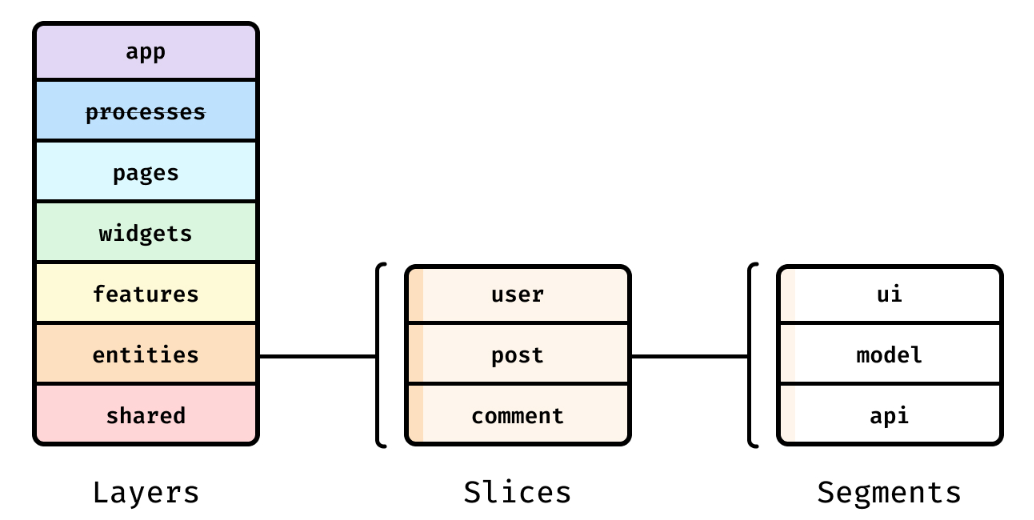
\includegraphics[scale=0.6]{styles/diploma/inc/fsd-pic1.png}
  \caption{Разделение проекта на слои, слайсы и сегменты}
  \label{fig:fsd}
\end{figure}

Данная методология обладает рядом преимуществ, которые делают его эффективным подходом для разработки фронтенд-проектов:

\begin{itemize}
    \item Архитектура FSD сосредоточена на бизнес-функциональности и разделяет код по функциональным возможностям. Это позволяет лучше структурировать и организовать код, делая бизнес-логику явной и понятной для разработчиков.
    \item Методология обеспечивает гибкость и адаптивность архитектуры. Компоненты могут быть легко заменены или добавлены в соответствии с новыми требованиями или условиями проекта. Это позволяет проекту быть более масштабируемым и способствует более простому внесению изменений.
    \item Архитектура FSD состоит из доменных модулей, таких как слои, слайсы и сегменты, что делает ее относительно простой для изучения и понимания. Разработчики могут быстро ориентироваться в структуре проекта и находить нужные модули, что способствует более эффективному сотрудничеству в команде.
    \item Благодаря структурированному подходу FSD, каждый модуль может быть независимо модифицирован или переписан без сайд-эффектов на другие модули. Это помогает управлять техническим долгом проекта и делает его более гибким для будущих изменений и развития.
    \item FSD находит баланс между принципом "Don't Repeat Yourself" (DRY) и локальной кастомизацией. Архитектура позволяет переиспользовать компоненты и модули, сохраняя при этом возможность их локальной настройки и кастомизации для конкретных потребностей проекта.
\end{itemize}

\subsubsection{Применение выбранной методологии в разработке}

Разработка по данной методологии начинается с определения и организации слоев. Каждый слой представляет собой логическую группировку модулей с определенными функциональными обязанностями. Слои включают shared, entities, features, widgets, pages, processes и app.

Рассмотрим алгоритм декомпозиции проекта на указанные слои по зонам ответственности. Когда разрабатывается новый модуль, разработчику необходимо определить к какому слою он должен относится. Представленные вопросы помогают отнести нужный модуль к нужному слою:

\begin{itemize}
    \item Shared: Это не относится к Бизнес-Логике и является общим переиспользуемым служебным кодом?
    \item Entities: Это относится непосредственно к бизнес-сущности?
    \item Features: Это относится к действию пользователя, представляющему бизнес-ценность?
    \item Widgets: Это самостоятельный и полноценный блок страницы с конкрытными действиями?
    \item Pages: Это относится к конкретной странице/экрану?
    \item Processes: Это относится к конкретному юзкейсу, протекающему через несколько страниц?
    \item App: Это общая инициализирующая логика приложения?
\end{itemize}

Рассмотрим каждый слой, отнеся к нему какой-нибудь модуль:

Shared: здесь располагаются переиспользуемые компоненты, например: кнопки, тексты, иконки, спиннеры, настройки безопасности, инстансы Axios, хуки, хелперы для работы со Store и т.д. Иными словами, компоненты без привязки к бизнес-логике. Пример представлен на рисунке~\ref{fig:fsd-shared}

\begin{figure}
  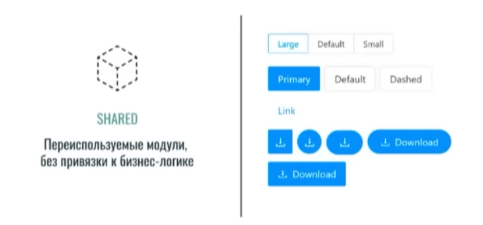
\includegraphics[scale=1]{styles/diploma/inc/fsd-shared.png}
  \caption{Слой Shared}
  \label{fig:fsd-shared}
\end{figure}

Entities: например карточка поста в соц-сети, на которой представленны только общие части, специфичные для всех постов. Функциональностей по типу лайков, вспомогательных кнопок, кнопки поделится и т.д., здесь не представлены. Они представлены в виде слотов, куда функциональности добавляются уже на уровне выше. Пример представлен на рисунке~\ref{fig:fsd-entities}

\begin{figure}
  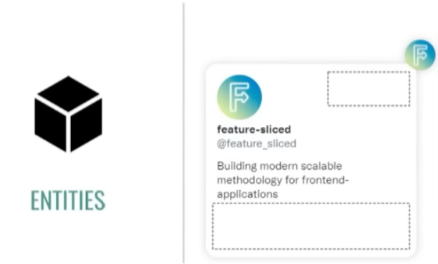
\includegraphics[scale=1]{styles/diploma/inc/fsd-entities.png}
  \caption{Слой Entities}
  \label{fig:fsd-entities}
\end{figure}

Features: здесь уже появляются функциональности, которые несут в себе какой-то бизнес-функционал, который приводит к какому-то результату, например: лайки, кнопка подписаться и т.д. Причем одна фича должна решать одну задачу. Пример представлен на рисунке~\ref{fig:fsd-features}

\begin{figure}
  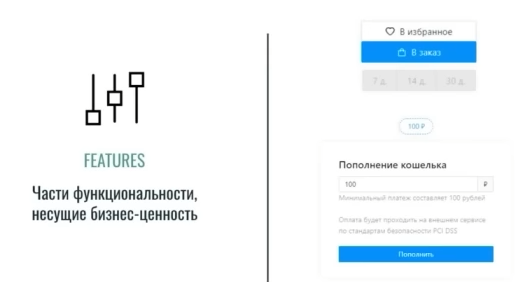
\includegraphics[scale=1]{styles/diploma/inc/fsd-features.png}
  \caption{Слой Features}
  \label{fig:fsd-features}
\end{figure}

Widgets: это комбинация entities, которые содержат "пустые слоты" и в эти слоты подставляются необходимые фичи (features). В данном случае, виджеты - это самостоятельные смысловые блоки, комбинирующие нижние слои. Полноценный пост, который можно оставить в группе - это уже виджет, причем один виджет может называть userPost, а другой groupPost, потому что с точки зрения функционала и работы с Backend они скорее всего будут разными. Пример представлен на рисунке~\ref{fig:fsd-widgets}

\begin{figure}
  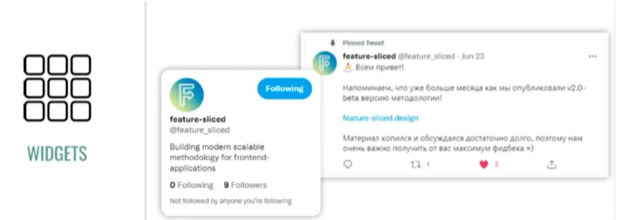
\includegraphics[scale=1]{styles/diploma/inc/fsd-widgets.png}
  \caption{Слой Widgets}
  \label{fig:fsd-widgets}
\end{figure}

Pages: страница собирается непосредственно из виджетов. Непосредственно в данном слои находится минимум бизнес-логики, запросов и прочего, все необходимое выносится на слои ниже. Пример представлен на рисунке~\ref{fig:fsd-pages}

\begin{figure}
  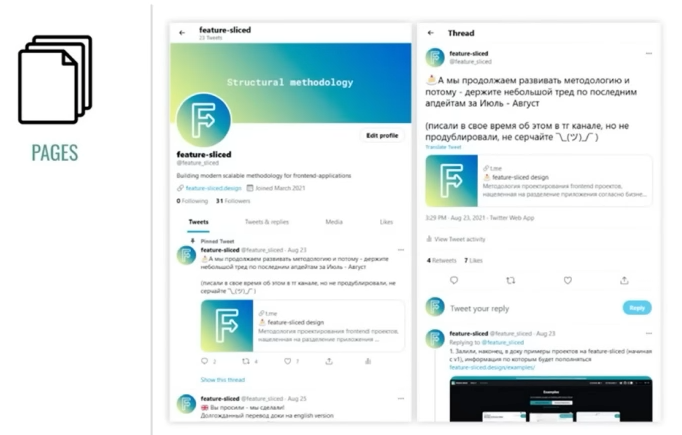
\includegraphics[scale=0.8]{styles/diploma/inc/fsd-pages.png}
  \caption{Слой Pages}
  \label{fig:fsd-pages}
\end{figure}

Processes: в нем хранится какой-то сложный набор действий, который протекает через несколько страниц. Например авторизация в несколько страниц.

App: данный слой хранит в себе инициализирующую логику приложения (Инициализирующая точка входа в приложение). Здесь хранятся все роутинг, провайдеры, глобальные стили, глобальные типы и все что не будет никогда и ни при каких условиях использоваться где-то ниже

    \section{РЕАЛИЗАЦИЯ КЛИЕНТСКОЙ ЧАСТИ}

\subsection{Реализация функционала заполнения и сохранения карт вызова}

Функционал заполнения и сохранения карт вызова представляет собой важную часть медицинского приложения, которое позволяет медицинским работникам эффективно вести медицинскую документацию и сохранять данные о пациентах. Перед реализацией функционала заполнения, необходимо подробно рассмотреть обратную сторону карты вызова, рисунок~\ref{fig:medical-card} .Для удобства навигации и промежуточного сохранения заполненных полей карта вызова должна быть разделена на несколько разделов.

Первым является раздел  - "Жалобы и Анамнез" - предназначен для заполнения данных о жалобах пациента и его медицинском анамнезе. Здесь медицинский работник может внести подробности, симптомы и предыдущую медицинскую историю пациента.

Следующий раздел - "Объективно" - предназначен для ввода объективных данных, полученных в результате осмотра пациента. Здесь могут быть указаны физические параметры, результаты осмотра органов и систем пациента.

Затем идут разделы, посвященные различным системам органов, такие как "Органы Дыхания", "Органы кровообращения", "Органы Пищеварения", "Нервная Система", "Костная Система". В каждом из этих разделов можно внести подробности о соответствующей системе органов пациента, включая симптомы, результаты исследований и т.д.

В разделе "Status Localis" заполняются основные данные о пациенте, такие как вес, пол, рост, возраст. Эти данные могут быть переданы модулям "Калькулятор дозировок" и "Таблицы Дифференциальной диагностики" через инструмент Redux, чтобы обеспечить удобную работу с этими данными в указанных модулях.

В разделе "Данные инструментальных исследований" может быть реализована функция загрузки фотографии снимка ЭКГ. После загрузки фотографии она может быть отправлена на сервер для обработки модулем "Острые патологии по снимку ЭКГ". Это позволит медицинскому персоналу быстро анализировать и диагностировать патологии на основе снимков ЭКГ.

В разделе "Оказанная помощь, ее эффект и рекомендации" необходимо указать информацию о предоставленной медицинской помощи, ее результаты и рекомендации для пациента.

И, наконец, раздел "Расходные материалы" предназначен для внесения информации о расходных материалах, использованных при оказании медицинской помощи.

Каждый раздел имеет множество полей, которые заполняются медицинским работником в соответствии с конкретной ситуацией и состоянием пациента. Для обеспечения более быстрого заполнения карты вызова необходимо проанализировать заполненные поля уже заполненных карт и выявить часто встречающиеся ответы. На основе этого анализа необходимо реализовать дополнительный функционал быстрых ответов, который предложит предварительно заполненные часто используемые значения для данных полей, что значительно ускорит процесс заполнения карты вызова. Промежуточный результат разработки заполнения карты вызова можно увидеть на рисунке~\ref{fig:result1}

\begin{figure}
  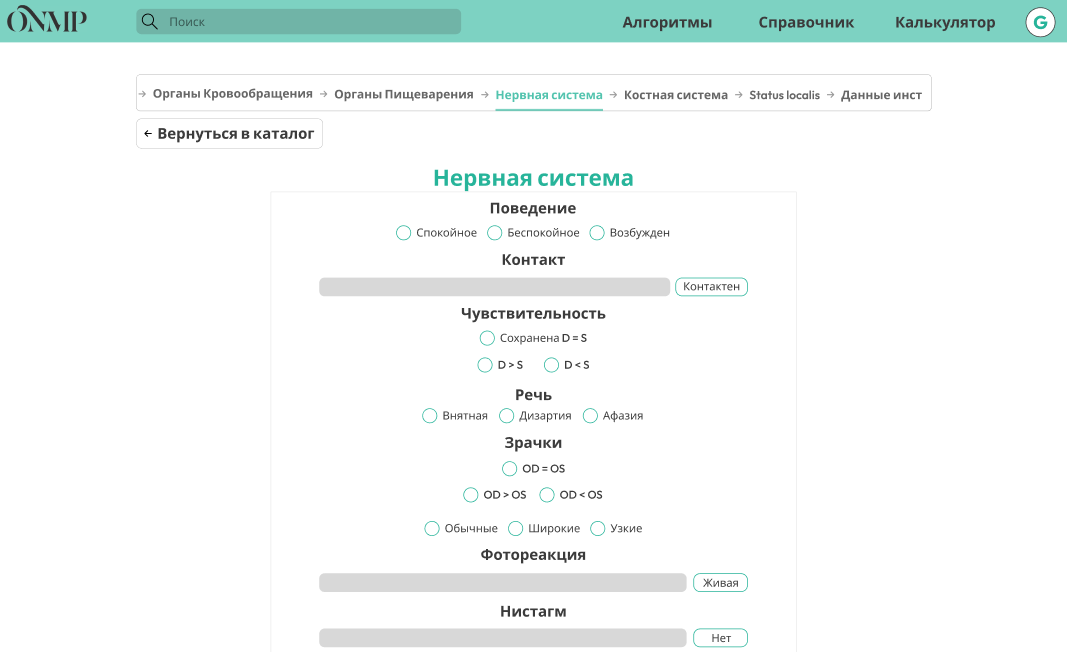
\includegraphics[scale=0.58]{styles/diploma/inc/result1.png}
  \caption{Страница заполнения карты вызова}
  \label{fig:result1}
\end{figure}

В результате реализации функционала заполнения и сохранения карт вызова в соответствии с описанными разделами, медицинские работники смогут эффективно и точно вести медицинскую документацию, сохранять данные о пациентах и облегчить себе работу при последующих визитах или обращениях пациентов.

\subsection{Разработка функционала организации папок и использования шаблонов}

Функционал организации папок и использования шаблонов для карт вызова обеспечивает максимальную эффективность и удобство использования. Разработка этого функционала включает создание четырех папок: Готовые, Незавершенные, Архив и Шаблоны.

В папку "Готовые" попадают карты вызова после того, как пользователь успешно заполнил все необходимые поля и нажал кнопку "Сохранить". Такая организация позволяет пользователям легко находить готовые карты вызова и быстро получать доступ к информации о каждом вызове.

В папку "Незавершенные" попадают карты вызова, когда пользователь не завершает их заполнение, например, закрывает вкладку или не нажимает кнопку "Сохранить". Однако уже введенные данные сохраняются в базе данных в процессе заполнения, чтобы пользователь мог возобновить работу с того места, где он остановился. Это обеспечивает сохранность введенных данных и позволяет избежать необходимости повторного заполнения всех полей.

В папку "Архив" перемещаются карты вызова после их распечатки или выполнения других действий, указанных пользователем. Архивирование карт вызова обеспечивает сохранность уже готовых карт, которые могут быть полезными для последующего анализа статистики, отчетов и других целей.

Папка "Шаблоны" предоставляет возможность создания базовых шаблонов карт вызова с частичным заполнением полей. Пользователи могут создавать шаблоны с предварительно заполненными данными, которые могут быть использованы в будущем как основа для создания новых карт вызова. Это существенно ускоряет процесс заполнения карт, поскольку многие поля уже будут заполнены заранее, и пользователю останется только внести дополнительную информацию. В результате, пользователи смогут более эффективно использовать время при заполнении карт вызова и уменьшить вероятность ошибок. Промежуточный результат разработки списка карт можно увидеть на рисунке~\ref{fig:result2}

\begin{figure}
  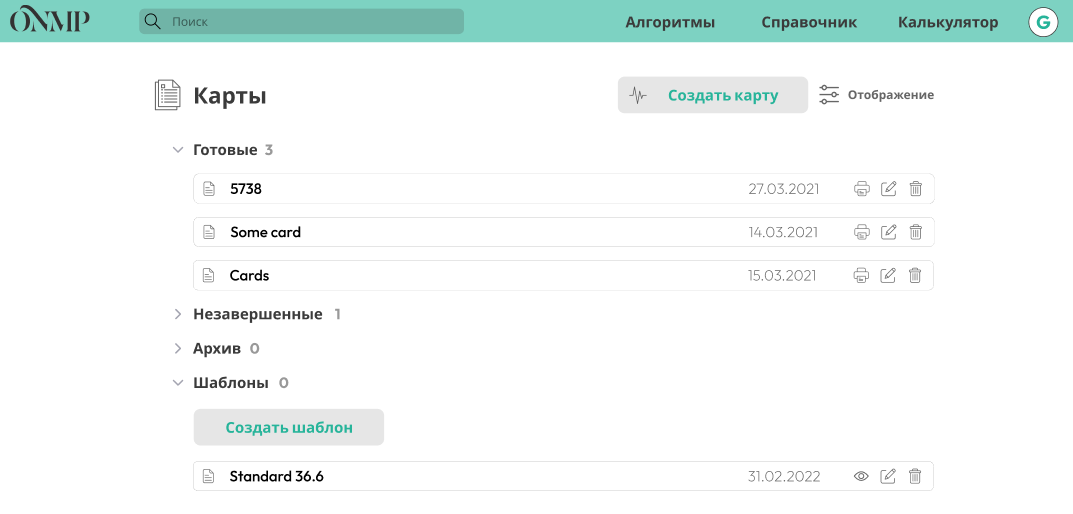
\includegraphics[scale=0.58]{styles/diploma/inc/result2.png}
  \caption{Страница со списком созданных карт}
  \label{fig:result2}
\end{figure}

Реализация функционала организации папок и шаблонов обеспечивает структурированный подход к хранению и управлению картами вызова, улучшает доступность и обработку данных, а также повышает эффективность работы с ними. Это существенно упрощает процесс работы медицинского персонала и повышает общую производительность системы.

    
    \conclusion

В ходе выполнения работы были достигнуты следующие результаты:

В ходе разработки клиентской части web-сервиса был реализован функционал, позволяющий пользователям заполнять карты вызова с учетом всех необходимых данных и сохранять их в соответствующих папках. Были созданы разделы для удобства навигации внутри карты и промежуточного сохранения заполненных полей. Также был разработан функционал организации папок и использования шаблонов, позволяющий пользователям быстро находить готовые карты вызова, восстанавливать незавершенные и архивировать уже выполненные карты. Внедрение данного функционала значительно упрощает и ускоряет процесс работы медицинского персонала, обеспечивая сохранность и доступность данных.

Оценивая полноту решений поставленных задач, можно сделать вывод о том, что в разработанной клиентской части web-сервиса были учтены основные требования к функциональности и удобству использования. Пользователи получили возможность удобно заполнять и сохранять карты вызова, а также организовывать их хранение с помощью папок и шаблонов. Разделение карт на разные разделы облегчает навигацию и повышает эффективность работы с системой.

В разработанной системе реализован функционал передачи данных модулям "Калькулятор дозировок" и "Таблицы Дифференциальной диагностики" на основе заполненных полей "status localis". Это обеспечивает более точные расчеты и диагностические рекомендации, основываясь на данных, введенных пользователем.

Рекомендации по использованию результатов работы включают в себя обучение персонала по использованию разработанной системы, создание документации с подробным описанием функционала и инструкциями по его использованию, а также обеспечение технической поддержки для пользователей системы. Дальнейшее развитие системы может включать расширение функционала, добавление новых модулей и интеграцию с другими системами здравоохранения.

Оценка технико-экономической эффективности внедрения разработанной системы показывает потенциал снижения временных затрат на заполнение и сохранение карт вызова. Автоматизация процесса заполнения и возможность использования шаблонов значительно повышают эффективность работы медицинского персонала. Кроме того, система обеспечивает удобство хранения и поиск готовых карт вызова, что способствует повышению производительности и снижению риска потери информации.

Сравнивая выполненную работу с лучшими достижениями в области, можно сделать вывод, что разработанная клиентская часть web-сервиса обладает современным и удобным пользовательским интерфейсом, а также предоставляет широкий функционал для заполнения, сохранения и организации карт вызова. Она соответствует современным стандартам разработки клиентских приложений и предоставляет удобные инструменты для работы медицинского персонала.

В целом, выполненная работа представляет собой значимый вклад в область разработки систем здравоохранения и обладает высоким уровнем научно-технического достижения. Разработанный функционал позволяет эффективно заполнять и сохранять карты вызова, повышая производительность и качество оказываемой медицинской помощи. Дальнейшее развитие и совершенствование системы могут вносить еще больший вклад в область здравоохранения и улучшать условия работы медицинских специалистов. % Заключение

    \printbibliography % Список литературы

    \appendix % Приложения
    \appendixsection{Карта вызова ОНМПВ и ДН}

Представленная карта карта вызова на рисунке~\ref{fig:medical-card} является приложением №6 к приказу Департамента здравоохранения города Москвы от 24 мая 2017 года №372\cite{appendix6}.


\begin{figure}
  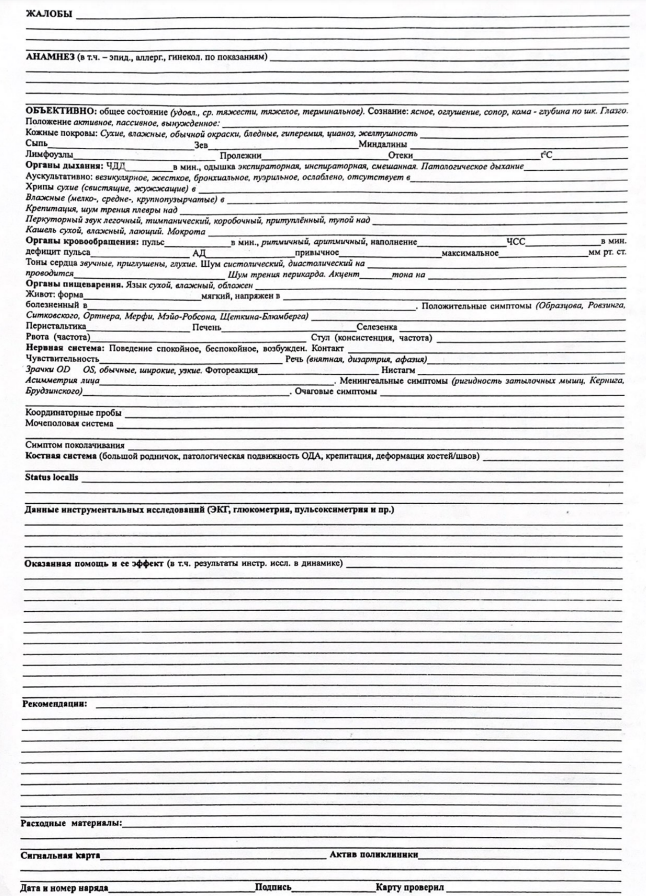
\includegraphics[scale=1]{styles/diploma/inc/medical-card.png}
  \caption{Карта вызова ОНМПВ и ДН}
  \label{fig:medical-card}
\end{figure}
\end{document}
